\section{espGG}

No último relatório deste projeto foi encontrado o código fonte da implementação do Grafo de Gabriel
utilizado na biblioteca GGClassification\footcite{https://CRAN.R-project.org/package=GGClassification}
disponível na plataforma CRAN\cite*{CRAN} para o linguagem R\cite*{Rlanguage}. 

A biblioteca foi implementada na linguagem C++ e utiliza uma interface com a linguagem R por meio das bibliotecas Rcpp\footcite{https://github.com/RcppCore/Rcpp}.
O código fonte da biblioteca pode ser encontrado no git:
\url{https://github.com/cran/GGClassification}

Dessa maneira, nessa etapa foi utilizado o código GGClassification como base para o desenvolvimento do projeto espGG, ou seja, a implementação do grafo de Gabriel em um microcontrolador esp32.

Utilizando os dados de um dos exemplos disponível na documentação do GGClassification vemos na seguinte imagem os resultados da saída serial do microcontrolador.

\begin{figure}[h!]
    \centering
    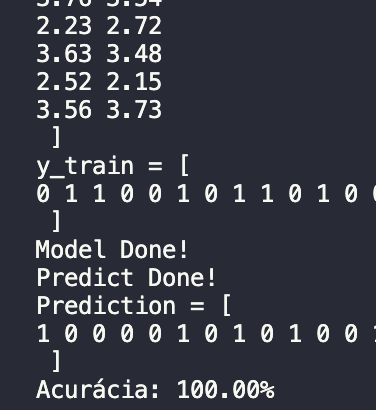
\includegraphics[scale=0.4]{images/espGGserial.png}
    \caption{Resultados do teste realizado.}
\end{figure}
